\section{Raster Operations}
\label{sec:raster-ops}
In \ref{sec:dispmanagement} we introduced the display area as an abstract concept, modeled as
a 2-dimensional Cartesian plane. So far, this view of the display space was sufficient
because we were interested in its global structure only and ignored contents completely. However,
if we are interested in what is displayed, we need to reveal more details about the model.

The Cartesian plane representing the display area is discrete. We consider points in the display
area as grid points or picture elements (\emph{pixel}), and we assume contents to be generated
by assigning colors to the pixels. For the moment, the number of possible colors a pixel can attain
is irrelevant. In the binary case of 2 colors we think of one representing background color
and the other foreground color.

The most elementary operation generating contents in a discrete plane is "set color of pixel"
or "set pixel" for short. While a few drawing algorithms directly build on this atomic operation,
block-oriented functionality (traditionally called \emph{raster operations})
plays a much more important role in practice. A \emph{block} is a rectangular area of pixels
whose bounding lines are parallel to the axes of the coordinate system.

Raster operations are based on a common principle:
\begin{itemize}
  \item A source block of width \verb|SW| and height \verb|SH| is placed at a given destination point
    \verb|(DX, DY)| in the display area.
  \item In the simplest case, the destination block \verb|(DX, DY, SW, SH)| is plainly overwritten
    by the source one.
  \item In general, the new value of each pixel in the destination block is a combination
    of its old value and the value of the corresponding source pixel:

    \[ d := F(s, d) \]
    
    $F$ is sometimes called the combination mode of the raster operation.  The raster is stored
    as an array of values of type \verb|SET|, each set representing 32 black/white pixels.
    The modes of combining source and destination is implemented by the following set operations:
    \begin{table}[h!]
      \centering
      \begin{tabular}{l l}
        mode           & operation \\\hline
        \verb|replace| & \verb|s| \\
        \verb|paint|   & \verb|s + d| (or) \\
        \verb|invert|  & \verb|s / d| (xor)
      \end{tabular}
    \end{table}
    \\Note that \verb|invert| is equivalent with inverse video mode if \verb|s| is
    \verb|TRUE| for all pixels.  There are many different variants of raster operations.
    Some refer to a source block in the display area, others specify a constant pattern
    to be taken as source block.  Some variants require replication of the source block
    within a given destination block \verb|(DX, DY, DW, DH)| rather than simple placement.
\end{itemize}

The challenge when designing a raster interface is finding a unified, small and complete set
of raster operations that covers all needs, in particular including the need of placing
character glyphs. The amazingly compact resulting set of Oberon raster operations
is exported by module \verb|Display|:
\begin{verbatim}
DEFINITION Display;
  CONST black = 0; white = 1;         (*colors*)
        replace = 0; paint = 1; invert = 2;
                             (*operation modes*)
  PROC Dot        (col,         x,y,     mode: INT);
  PROC ReplConst  (col,         x,y,w,h, mode: INT);
  PROC CopyBlock  (sx,sy, w,h, dx,dy,    mode: INT);
  PROC CopyPattern(col, patadr, x,y,     mode: INT);
  PROC ReplPattern(col, patadr, x,y,w,h, mode: INT);
END Display.
\end{verbatim}
In the parameter lists of the above raster operations,
\verb|mode| is the mode of combination (\verb|replace|, \verb|paint|, or \verb|invert|).
\verb|CopyBlock| copies the source block \verb|(sx, sy, w, h)| to position \verb|(dx, dy)|
and uses \verb|mode| to combine new contents in the destination block \verb|(dx, dy, w, h)|.
It is assumed tacitly that the numbers of colors per pixel
in the source block and in the destination area are identical.
It is perhaps informative to know that \verb|CopyBlock| is essentially equivalent
with the famous \verb|BitBlt| (bit block transfer) in the SmallTalk project \cite{Goldberg}.
In Oberon, it is used primarily for scrolling contents within a viewer.

The remaining raster operations use a constant pattern.
Patterns are implemented as arrays of bytes, and the parameter
\verb|patadr| is the address of the relevant pattern.
The 1st 2 bytes indicate width \verb|w| and height \verb|h| of the pattern.
Pattern data are given as a sequence of bytes to be placed into the destination block
from left to right and from bottom to top. Each line takes an integral number of bytes.
Hence, the number of data bytes is $((w+7) / 8) * h$. Fig \ref{fig:pattern} shows an example:
\begin{figure}[h!]
  \centering
  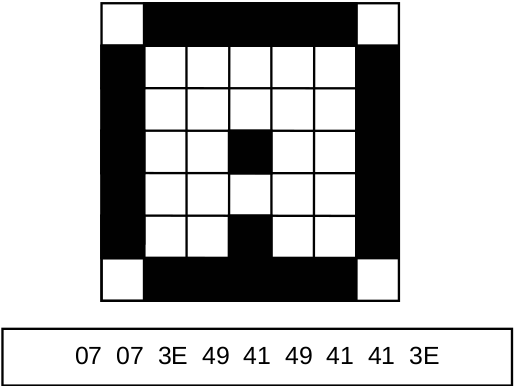
\includegraphics[width=.6\textwidth]{i/b}
  \caption{A pattern and its encoding as an array of bytes (in hex)}
  \label{fig:pattern}
\end{figure}

Some standard patterns are included in module \verb|Display| and exported as global variables.
Among them
\begin{table}[h!]
  \centering
  \begin{tabular}{l l}
    patterns  & intended to represent \\\hline
    arrow,    & the cursor, \\
    hook, and & the caret, and \\
    star      & the marker.
  \end{tabular}
\end{table}
\\A group of predefined patterns supports drawing graphics.
\begin{itemize}
  \item \verb|col| in the pattern-oriented raster operations specifies the pattern's foreground color.
    Colors black (background) and white are predefined.
  \item \verb|CopyPattern| copies the pattern to location \verb|x|, \verb|y| in the display area,
    using the given combination mode.
    It is probably the most frequently used operation of all because it is needed to write text.
  \item \verb|ReplPattern| replicates the given pattern to the given destination block.
    It starts at bottom left and proceeds from left to right and from bottom to top.
  \item \verb|Dot| and \verb|ReplConst| are special cases of \verb|CopyPattern| and \verb|ReplPattern|
    respectively, taking a fixed implicit pattern consisting of a single foreground pixel.
    \begin{itemize}
      \item \verb|Dot| is exactly our previously mentioned "set pixel".
      \item \verb|ReplConst| is used to draw horizontal and vertical lines of various widths.
    \end{itemize}
\end{itemize}

The raster operations are a prominent example of the use of Oberon's data type \verb|SET|.
Formally, variables are sets of integers between 0 and 31.
Here, they are taken as sets of bits numbered from 0 to 31.
We consider the replication of 1's (\verb|mode| = \verb|replace| or \verb|paint|)
in the rectangle with origin \verb|x|, \verb|y|, width \verb|w|, and height \verb|h|.
Every line consists of 1024 pixels, or 32 words.
\verb|al|, \verb|ar|, \verb|a0|, \verb|a1| are addresses.
\begin{verbatim}
  VAR al, ar, a0, a1: INT;
      left, right, pixl, pixr: SET;
  
  al := base + y*128;
  ar := ((x+w-1) DIV 32)*4 + al;
  al := (x DIV 32)*4 + al;
  left  := {(x MOD 32) .. 31};
  right := {0 .. ((x+w-1) MOD 32)};
  FOR a0 := al TO al + (h-1)*128 BY 128 DO
    SYSTEM.GET(a0, pixl);
    SYSTEM.GET(ar, pixr);
    SYSTEM.PUT(a0, pixl + left);
    FOR a1 := a0+4 TO ar-4 BY 4 DO
      SYSTEM.PUT(a1, {0 .. 31});
    END
    SYSTEM.PUT(ar, pixr + right)
  END
\end{verbatim}
The definition (and even more so the implementation) of module \verb|Display| provides support
for a restricted class of possible hardware configurations only. Any number of display monitors
is theoretically possible. However, they must be mapped to a regular horizontal array
of predefined cells in the display area. Each cell is vertically split into 2 congruent regions,
where the corresponding monitor is supposed to be able to select and display one of the 2 regions
alternatively. Finally, it is assumed that all cells hosting black-and-white monitors
are allocated to the left of all cells hosting color monitors.
Fig \ref{fig:cell} gives an impression of such a configuration.
\begin{figure}[h!]
  \centering
  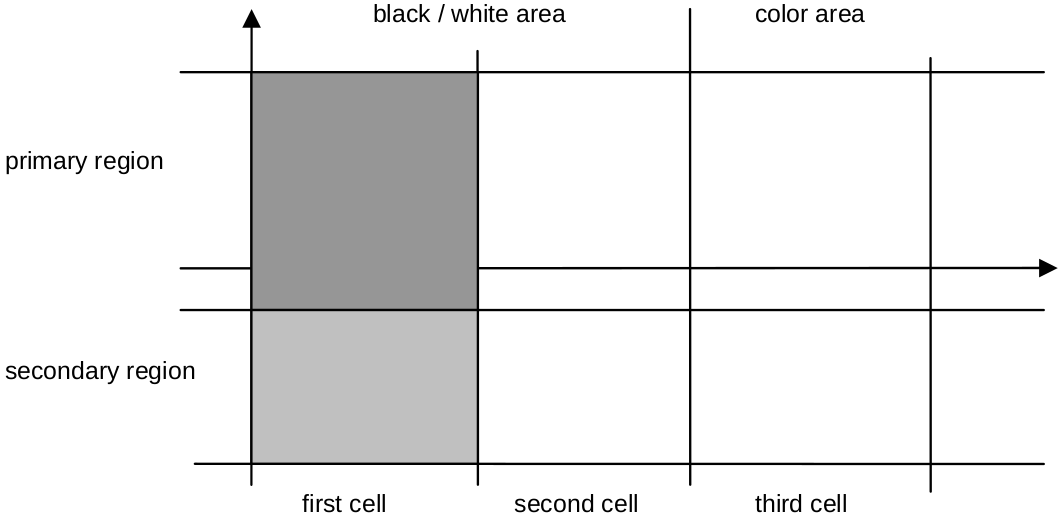
\includegraphics[width=\textwidth]{i/c}
  \caption{General, regular cell structure of display area}
  \label{fig:cell}
\end{figure}

Under these restrictions any concrete configuration can be parameterized by the variables
of the definition above. \verb|Unit|, \verb|Width|, and \verb|Height| specify the extent
of a displayed region, where \verb|Width| and \verb|Height| are width and height in pixel units,
and \verb|Unit| is the size of a pixel in units of 1/36’000 mm.  This unit is a common divisor
of all of the standard metric units used by the typesetting community, like mm, inch, Pica point
and point size of usual printing devices.  \verb|Bottom| and \verb|UBottom| specify
the bottom y-coordinate of the primary region and the secondary region respectively.
Finally, \verb|Left| and \verb|ColLeft| give the left x-coordinate of the area
of black-and-white monitors and of color monitors respectively.
